\chapter{状态空间模型}

\section{从结构图或电路列状态方程}

\ex{习题1（习题课第1页）\quad RLC 电路建模}{
如图，RLC 电路中含电压源 $u_1(t)$ 和电流源 $u_2(t)$。试建立以两源为输入、电感 $L$ 上的电压 $u_L(t)$ 为输出的状态空间模型。
\par\smallskip
\begin{center}
    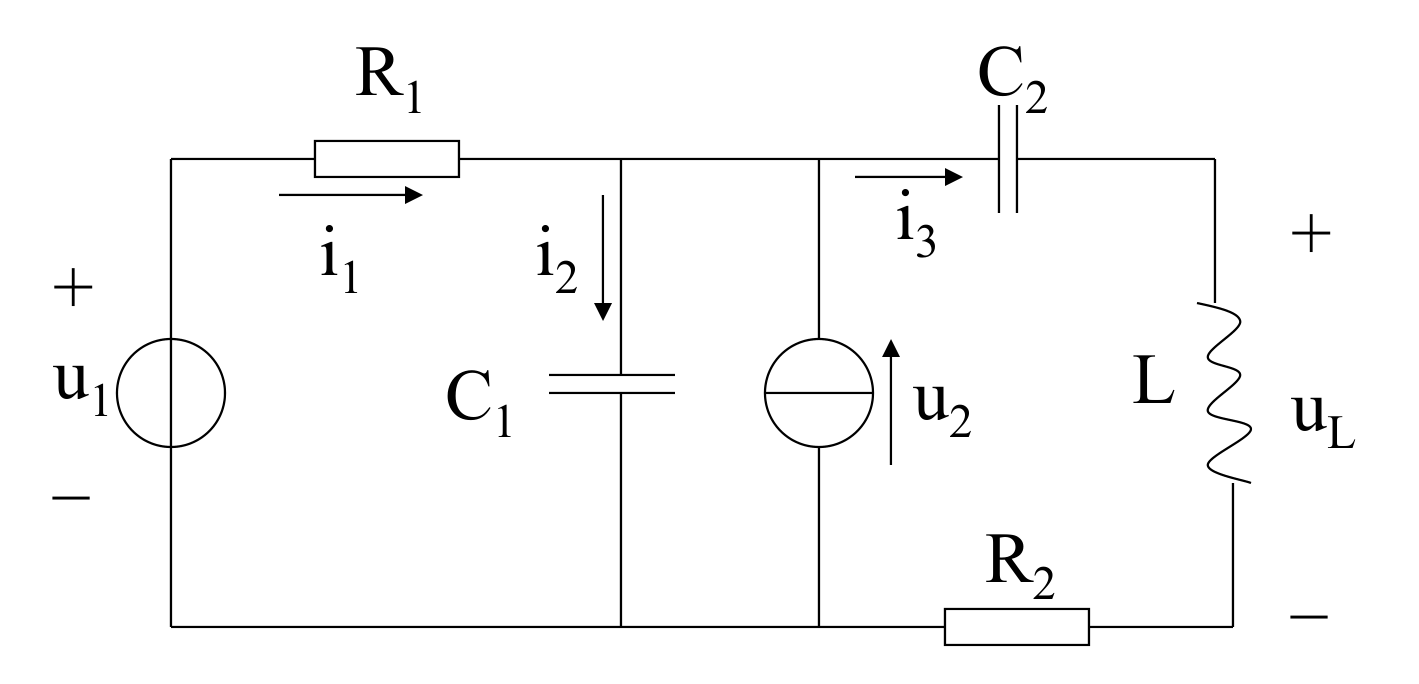
\includegraphics[width=0.61\linewidth]{ch02-rlc-circuit.png}
\end{center}
}

\nt{\textbf{解题顺序}\quad 标出电容电压极性及支路电流，写上方节点的 KCL，再写右侧回路的 KVL，最后整理为矩阵。}

\sol 令 $x_1=u_{C_1}$（上正下负）、$x_2=u_{C_2}$（左正右负）、$x_3=i_3$，$u=[u_1,u_2]^{\mathsf T}$。电流源箭头朝上，所以在电路上方的公共节点有 $i_1+u_2=i_2+i_3$。左支路给出 $i_1=(u_1-x_1)/R_1$，而 $i_2=C_1\dot x_1$，因此
\[
C_1\dot x_1=\frac{u_1-x_1}{R_1}+u_2-x_3.
\]
从右支路可读出 $C_2\dot x_2=x_3$。沿 $C_2$、$L$、$R_2$ 所在回路列电压方程，得
\[
x_1=x_2+u_L+R_2x_3,\qquad u_L=L\dot x_3.
\]
逐式除以储能元件参数，得到
\[
\dot x_1=-\frac{x_1}{R_1C_1}-\frac{x_3}{C_1}
             +\frac{u_1}{R_1C_1}+\frac{u_2}{C_1},\quad
\dot x_2=\frac{x_3}{C_2},\quad
\dot x_3=\frac{x_1-x_2-R_2x_3}{L}.
\]
按 $x_1,x_2,x_3$ 和 $u_1,u_2$ 的顺序读出系数，得
\[
\dot x=
\begin{bmatrix}
-\frac1{R_1C_1}&0&-\frac1{C_1}\\
0&0&\frac1{C_2}\\
\frac1L&-\frac1L&-\frac{R_2}L
\end{bmatrix}x+
\begin{bmatrix}
\frac1{R_1C_1}&\frac1{C_1}\\
0&0\\
0&0
\end{bmatrix}u,\qquad
y=\begin{bmatrix}1&-1&-R_2\end{bmatrix}x.
\]
输出由三个状态量直接求得，故 $D=[0\quad 0]$。

\ex{纸质练习一\quad 由反馈结构图建立状态空间模型}{
按图中的 $x_1,x_2$ 选取状态，求输入 $u$ 到输出 $y$ 的状态空间表达式。
\begin{center}
\begin{tikzpicture}[>=Stealth,
    block/.style={draw, minimum width=1.65cm, minimum height=0.95cm},
    sum/.style={draw,circle,inner sep=0pt,minimum size=6mm}]
    \node[sum] (sum) at (0,0) {$\scriptstyle\sum$};
    \node[block] (plant) at (2.35,0) {$\dfrac{k}{s+2}$};
    \node[block] (sensor) at (2.35,-1.4) {$\dfrac{1}{s+1}$};
    \draw[->] (-1.4,0) node[above] {$u$} -- node[above,pos=.82] {$+$} (sum);
    \draw[->] (sum) -- (plant);
    \draw[->] (plant) -- (4.9,0) node[right] {$y$};
    \fill (3.9,0) circle[radius=1.2pt] node[above] {$x_1$};
    \draw[->] (3.9,0) |- (sensor.east);
    \draw[->] (sensor.west) -| node[pos=.3,above] {$x_2$}
        node[pos=.86,right] {$-$} (sum.south);
\end{tikzpicture}
\end{center}
}

\nt{\textbf{解题顺序}\quad 圈出 $x_1,x_2$，从反馈求和点读出 $u-x_2$，把每个分母移到该环节的等式左边。}

\sol 先读求和点。前向环节的输入为 $u-x_2$，其输出为 $x_1$。反馈环节的输入为 $x_1$，输出为 $x_2$，因此在时域中有
\[
    \dot x_1+2x_1=k(u-x_2),\qquad \dot x_2+x_2=x_1.
\]
输出从前向环节末端引出，故 $y=x_1$。整理得
\[
    \boxed{
    \dot x=\begin{bmatrix}-2&-k\\1&-1\end{bmatrix}x
           +\begin{bmatrix}k\\0\end{bmatrix}u,\qquad
    y=\begin{bmatrix}1&0\end{bmatrix}x,\quad D=0.}
\]
检验时可在零初始条件下消去 $X_2=X_1/(s+1)$，得到
\[
    \frac{Y(s)}{U(s)}=\frac{k(s+1)}{(s+2)(s+1)+k}.
\]

\ex{讲义例2-1（第25--26页）\quad 由模型画模拟结构图}{
已知
\[
\dot x=\begin{bmatrix}0&a&0\\0&b&c\\d&0&e\end{bmatrix}x+
\begin{bmatrix}0\\0\\f\end{bmatrix}u,\qquad
y=\begin{bmatrix}1&0&0\end{bmatrix}x.
\]
画出模拟结构图，并从图反读其状态方程。}

\nt{\textbf{解题顺序}\quad 先列三个状态分量的等式，再将各等式右边的和接到对应积分器。}

\sol 从最后一个状态开始，$fu$、$dx_1$ 与 $ex_3$ 先相加，经积分器得到 $x_3$。$cx_3+bx_2$ 积分得到 $x_2$，$ax_2$ 积分得到 $x_1$，直接取 $y=x_1$。
\begin{center}
\begin{tikzpicture}[>=Stealth,block/.style={draw,minimum width=7mm,minimum height=6mm},
    sum/.style={draw,circle,inner sep=0pt,minimum size=5mm}]
    \node[block] (f) at (.75,0) {$f$};
    \node[sum] (s3) at (1.55,0) {$+$};
    \node[block] (i3) at (2.6,0) {$\int$};
    \node[block] (c) at (3.85,0) {$c$};
    \node[sum] (s2) at (4.65,0) {$+$};
    \node[block] (i2) at (5.7,0) {$\int$};
    \node[block] (a) at (6.95,0) {$a$};
    \node[block] (i1) at (8,0) {$\int$};
    \node[block] (e) at (2.4,-.9) {$e$};
    \node[block] (b) at (5.5,-.9) {$b$};
    \node[block] (d) at (5,1.05) {$d$};
    \draw[->] (0,0) node[left] {$u$} -- (f);
    \draw[->] (f) -- (s3);
    \draw[->] (s3) -- node[above] {$\dot x_3$} (i3);
    \draw[->] (i3) -- node[above] {$x_3$} (c);
    \draw[->] (c) -- (s2);
    \draw[->] (s2) -- node[above] {$\dot x_2$} (i2);
    \draw[->] (i2) -- node[above] {$x_2$} (a);
    \draw[->] (a) -- node[above] {$\dot x_1$} (i1);
    \draw[->] (i1) -- node[above] {$x_1$} (9.25,0) node[right] {$y$};
    \draw[->] (3.2,0) |- (e);
    \draw[->] (e) -| (s3);
    \draw[->] (6.3,0) |- (b);
    \draw[->] (b) -| (s2);
    \draw[->] (8.72,0) |- (d);
    \draw[->] (d) -| (s3);
    \foreach \x in {3.2,6.3,8.72} \fill (\x,0) circle[radius=1pt];
\end{tikzpicture}
\end{center}
沿三个积分器的输入端反查，分别得到 $\dot x_1=ax_2$、$\dot x_2=bx_2+cx_3$ 和 $\dot x_3=dx_1+ex_3+fu$。

\noindent\textbf{验算}\quad 两输入电路的 $B$ 有两列。若输出是电感电压，先用 $u_L=L\dot i_L$，再代入状态方程消去导数。

\section{从微分方程写状态空间模型}

\ex{习题2（习题课第5页）\quad 右端无输入导数的微分方程}{
已知 $y^{(3)}+5\ddot y+8\dot y+6y=3u$，求状态空间表达式。}

\nt{\textbf{解题顺序}\quad 取 $x_1=y,x_2=\dot y,x_3=\ddot y$，先写两条积分链，再移项求 $\dot x_3$。}

\sol 令 $x_1=y$、$x_2=\dot y$、$x_3=\ddot y$，则 $\dot x_1=x_2$、$\dot x_2=x_3$，原方程解出 $\dot x_3=-6x_1-8x_2-5x_3+3u$。所以
\[
\dot x=
\begin{bmatrix}0&1&0\\0&0&1\\-6&-8&-5\end{bmatrix}x
+\begin{bmatrix}0\\0\\3\end{bmatrix}u,\qquad
y=\begin{bmatrix}1&0&0\end{bmatrix}x.
\]
矩阵最后一行的系数按 $y,\dot y,\ddot y$ 排列。初值对应为 $x(0)=[y(0),\dot y(0),\ddot y(0)]^{\mathsf T}$。

\ex{习题3（习题课第7页）\quad 右端含输入导数的微分方程}{
已知 $y^{(3)}+4\ddot y+2\dot y+y=\ddot u+\dot u+3u$，求状态空间表达式。}

\nt{\textbf{解题顺序}\quad 先设 $x_1=y$，逐级吸收输入导数。按 $\ddot u,\dot u,u$ 对齐系数，再组装 $B$。}

\sol 令 $x_1=y$、$\dot x_1=x_2+\beta_2 u$、$\dot x_2=x_3+\beta_1u$。这相当于取
\[
x_2=\dot y-\beta_2 u,\qquad
x_3=\ddot y-\beta_2\dot u-\beta_1 u.
\]
再令 $\dot x_3=-x_1-2x_2-4x_3+\beta_0u$。此时
\[
\dot y=x_2+\beta_2u,\quad
\ddot y=x_3+\beta_1u+\beta_2\dot u,\quad
y^{(3)}=\dot x_3+\beta_1\dot u+\beta_2\ddot u.
\]
代回左端，$x_1,x_2,x_3$ 项抵消，余下
\[
\beta_2\ddot u+(\beta_1+4\beta_2)\dot u+
(\beta_0+4\beta_1+2\beta_2)u.
\]
逐阶对齐系数得到 $\beta_2=1$、$\beta_1=1-4=-3$、$\beta_0=3-4(-3)-2=13$，因此
\[
\dot x=
\begin{bmatrix}0&1&0\\0&0&1\\-1&-2&-4\end{bmatrix}x+
\begin{bmatrix}1\\-3\\13\end{bmatrix}u,\qquad
y=\begin{bmatrix}1&0&0\end{bmatrix}x .
\]
零初值下，该模型的传递函数分子为 $s^2+s+3$、分母为 $s^3+4s^2+2s+1$。

\noindent\textbf{易错}\quad 矩阵末行由低阶到高阶填负系数。右端含输入导数时，直接令 $x_2=\dot y,x_3=\ddot y$ 会留下 $\dot u$ 或 $\ddot u$。

\section{传递函数与状态空间模型互换}

\ex{习题4（习题课第10页）\quad 由单极点求对角规范形}{
给定 $G(s)=(s^2+6s+8)/(s^2+4s+3)$，求对角规范形状态空间表达式。}

\nt{\textbf{解题顺序}\quad 分子与分母同阶，先长除取 $D$。剩余部分对两个单极点取留数，写成两个并联状态。}

\sol 分子与分母同阶且首项系数相同，长除得 $D=1$。因式分解后
\[
G(s)-1=\frac{2s+5}{(s+1)(s+3)}
=\frac{3/2}{s+1}+\frac{1/2}{s+3}.
\]
两个留数直接代入
\[
r_1=\left.\frac{2s+5}{s+3}\right|_{s=-1}=\frac32,\qquad
r_2=\left.\frac{2s+5}{s+1}\right|_{s=-3}=\frac12.
\]令 $X_1/U=1/(s+1)$、$X_2/U=1/(s+3)$，可取
\[
\dot x=\begin{bmatrix}-1&0\\0&-3\end{bmatrix}x+
\begin{bmatrix}1\\1\end{bmatrix}u,\qquad
y=\begin{bmatrix}3/2&1/2\end{bmatrix}x+u.
\]
验算 $G(\infty)=D=1$。

\ex{习题5（习题课第12页）\quad 由重极点求约旦规范形}{
给定 $G(s)=(4s^2+10s+5)/(s^3+5s^2+8s+4)$，求约旦规范形状态空间表达式。}

\nt{\textbf{解题顺序}\quad 先因式分解。乘去重极点因子，用代入与求导分别算二次、一次分式系数。让输入进入约旦块最后一个状态。}

\sol 分母为 $(s+2)^2(s+1)$，故
\[
G(s)=\frac{\alpha}{(s+2)^2}+\frac{\beta}{s+2}+\frac{\gamma}{s+1}.
\]
记 $h(s)=(s+2)^2G(s)=(4s^2+10s+5)/(s+1)$。代入 $s=-2$，得 $\alpha=h(-2)=-1$。由于第三项乘 $(s+2)^2$ 后在 $s=-2$ 有二阶零点，只需对 $h$ 求导。记 $N(s)=4s^2+10s+5$，有 $N(-2)=1,N'(-2)=-6$。商法则给出
\[
\beta=h'(-2)=\frac{N'(-2)(-1)-N(-2)}{(-1)^2}=5,\qquad
\gamma=\left.\frac{N(s)}{(s+2)^2}\right|_{s=-1}=-1.
\]

令 $\dot x_2=-2x_2+u$，$\dot x_1=-2x_1+x_2$，则 $X_2/U=(s+2)^{-1}$、$X_1/U=(s+2)^{-2}$。再令 $\dot x_3=-x_3+u$。结合三个分式系数得到
\[
\dot x=\begin{bmatrix}-2&1&0\\0&-2&0\\0&0&-1\end{bmatrix}x+
\begin{bmatrix}0\\1\\1\end{bmatrix}u,\qquad
y=\begin{bmatrix}-1&5&-1\end{bmatrix}x .
\]

\ex{习题8／讲义例2-12（只差直联项）\quad 从状态空间求传递函数}{
已知
\[
\dot x=\begin{bmatrix}-5&-1\\3&-1\end{bmatrix}x+
\begin{bmatrix}2\\5\end{bmatrix}u,\qquad
y=\begin{bmatrix}1&2\end{bmatrix}x+Du.
\]
分别求 $D=0$（讲义例2-12，$y=[1\;2]x$）与 $D=4$（习题8，$y=[1\;2]x+4u$）时的传递函数。}

\nt{\textbf{解题顺序}\quad 求 $\det(sI-A)$ 与伴随矩阵，依次乘 $B,C$，最后加 $D$。}

\sol 先算
\[
sI-A=\begin{bmatrix}s+5&1\\-3&s+1\end{bmatrix},\qquad
(sI-A)^{-1}=\frac{1}{(s+2)(s+4)}
\begin{bmatrix}s+1&-1\\3&s+5\end{bmatrix}.
\]
将分子矩阵右乘 $B$，得到 $[2s-3,5s+31]^{\mathsf T}$。左乘 $C$ 后加相应直联项，可得
\[
G_{\text{例2-12}}(s)=\frac{12s+59}{(s+2)(s+4)},\qquad
G_{\text{习题8}}(s)=\frac{4s^2+36s+91}{s^2+6s+8}.
\]
由于在 $s=-2,-4$ 处严格真分式的分子均非零，加常数也不会消去这两个极点。高频极限分别为 $0$、$4$，与 $D$ 一致。

\noindent\textbf{验算}\quad 先核对 $D$ 与高频极限。二阶约旦块入口在最后一态，高次分式系数写在该块的输出首位。

\section{对角化与约旦规范形}

\ex{习题6／讲义例2-6（同一系统）\quad 相似变换到对角规范形}{
给定如下状态空间表达式。
\[
\dot x=
\begin{bmatrix}0&1&0\\0&0&1\\-6&-11&-6\end{bmatrix}x+
\begin{bmatrix}0\\0\\6\end{bmatrix}u,\qquad
y=\begin{bmatrix}1&0&0\end{bmatrix}x.
\]
讲义例2-6 给定变换矩阵 $P=\begin{bmatrix}1&1&1\\-1&-2&-3\\1&4&9\end{bmatrix}$，求变换后的模型。习题6 要求从原模型出发，求对角规范形。}

\nt{\textbf{解题顺序}\quad 按特征值排 $P$ 的列，先查 $AP=P\Lambda$，再算 $P^{-1}B$ 和 $CP$。}

\sol $\det(\lambda I-A)=\lambda^3+6\lambda^2+11\lambda+6=(\lambda+1)(\lambda+2)(\lambda+3)$。对于特征值 $\lambda$，$Ap=\lambda p$ 的前两行给出 $p_2=\lambda p_1$、$p_3=\lambda^2p_1$，末行由特征方程满足。取 $p_1=1$，按 $\lambda=-1,-2,-3$ 排列列向量，得到
\[
P=\begin{bmatrix}1&1&1\\-1&-2&-3\\1&4&9\end{bmatrix},\qquad
P^{-1}=\begin{bmatrix}3&5/2&1/2\\-3&-4&-1\\1&3/2&1/2\end{bmatrix}.
\]
这正是例2-6 给定的 $P$。从给定矩阵出发，可直接用 $AP=P\operatorname{diag}(-1,-2,-3)$ 核对各列。令 $z=P^{-1}x$，于是
\[
\dot z=\operatorname{diag}(-1,-2,-3)z+
\begin{bmatrix}3\\-6\\3\end{bmatrix}u,\qquad
y=\begin{bmatrix}1&1&1\end{bmatrix}z.
\]
$\bar C=CP$ 取 $P$ 的首行，$\bar B=P^{-1}B$ 等于 $P^{-1}$ 的末列乘 6。

\ex{习题7（习题课第17页）\quad 相似变换到约旦规范形}{
将下列状态方程化为约旦规范形。
\[
\dot x=\begin{bmatrix}4&1&-2\\1&0&2\\1&-1&3\end{bmatrix}x+
\begin{bmatrix}3&1\\2&7\\5&3\end{bmatrix}
\begin{bmatrix}u_1\\u_2\end{bmatrix}.
\]}

\nt{\textbf{解题顺序}\quad 先求重根的几何重数。选普通特征向量，再解 $(A-\lambda I)r=q$。按链排列 $P$ 后计算 $P^{-1}B$。}

\sol 展开 $\det(\lambda I-A)=\lambda^3-7\lambda^2+15\lambda-9=(\lambda-1)(\lambda-3)^2$。对 $\lambda=1$，$(A-I)p=0$ 的后两行给出 $p_1-p_2+2p_3=0$，再与第一行合用得 $p_1=0,\ p_2=2p_3$，取 $p=[0,2,1]^{\mathsf T}$。

对 $\lambda=3$，记
\[
N=A-3I=\begin{bmatrix}1&1&-2\\1&-3&2\\1&-1&0\end{bmatrix}.
\]
由第三行得 $q_1=q_2$，第一行再给出 $q_3=q_1$，所以 $\dim\ker N=1$，取 $q=[1,1,1]^{\mathsf T}$。解 $Nr=q$，第三行给 $r_1-r_2=1$，第一行给 $r_2=r_3$。令 $r_2=r_3=1$，则 $r=[2,1,1]^{\mathsf T}$，代回第二行得 $2-3+2=1$。

将普通特征向量放在广义特征向量前，取
\[
P=\begin{bmatrix}0&1&2\\2&1&1\\1&1&1\end{bmatrix},\qquad
P^{-1}=\begin{bmatrix}0&1&-1\\-1&-2&4\\1&1&-2\end{bmatrix}.
\]
由 $Ap=p$、$Aq=3q$、$Ar=q+3r$ 可直接读取 $\bar A$ 的各列。将 $B$ 的两列分别左乘 $P^{-1}$，得
\[
\dot z=\begin{bmatrix}1&0&0\\0&3&1\\0&0&3\end{bmatrix}z+
\begin{bmatrix}-3&4\\13&-3\\-5&2\end{bmatrix}
\begin{bmatrix}u_1\\u_2\end{bmatrix},\qquad z=P^{-1}x.
\]

\ex{讲义例2-8（第116--119页）\quad 三重特征值的两条链}{
求 $A=\begin{bmatrix}-4&-3&-6\\1&0&2\\1&1&1\end{bmatrix}$ 的特征向量及特征向量链。}

\nt{\textbf{解题顺序}\quad 设 $N=A+I$，算秩和 $N^2$，找一条长度为 2 的链，再补一个独立特征向量。}

\sol 令 $N=A+I$。其三行均是 $[1,1,2]$ 的倍数，故 $\rank N=1$，并有 $N^2=0$。因此只有特征值 $-1$，代数重数为 3，特征空间维数为 2。有一条长度为 2 的链和一条长度为 1 的链。取 $w=[1,0,1]^{\mathsf T}$，得 $Nw=[-9,3,3]^{\mathsf T}=v$ 且 $Nv=0$。再取 $q=[1,1,-1]^{\mathsf T}$，有 $Nq=0$，且 $q$ 与 $v$ 无比例关系。于是 $[v,w]$ 为长度为 2 的链，$[q]$ 为另一条链，$P=[v,w,q]$ 给出
\[
P^{-1}AP=\begin{bmatrix}-1&1&0\\0&-1&0\\0&0&-1\end{bmatrix}.
\]

\noindent\textbf{易错}\quad 取 $x=Pz$ 时，$\bar B=P^{-1}B$、$\bar C=CP$。约旦链先放普通向量，再放广义向量，顺序可用 $AP=PJ$ 核对。

\section{讲义指定题：读三积分器与构造约旦链}

\ex{教材图1.7(b)（讲义第26页）\quad 三积分器带负反馈}{
正向通道依次为 $K_1/(T_1s+1)$、$K_2/(T_2s+1)$、$K_3/(T_3s)$。输出经 $K_4$ 反馈到第一个求和点的负端。按图从左到右把各环节的输出取为 $x_3,x_2,x_1$，求状态方程和输出方程。
\begin{center}
\begin{tikzpicture}[>=Stealth,
    block/.style={draw=myb,fill=mytheorembg,minimum width=15mm,minimum height=8mm},
    sum/.style={draw,circle,minimum size=5mm,inner sep=0pt}]
    \node[sum] (sum) at (0,0) {$\scriptstyle\sum$};
    \node[block] (one) at (1.7,0) {$\dfrac{K_1}{T_1s+1}$};
    \node[block] (two) at (4.05,0) {$\dfrac{K_2}{T_2s+1}$};
    \node[block] (three) at (6.45,0) {$\dfrac{K_3}{T_3s}$};
    \node[block] (four) at (4.05,-.96) {$K_4$};
    \draw[->] (-1.04,0) node[left] {$u$} -- node[pos=.68,above] {$+$} (sum);
    \draw[->] (sum) -- node[above] {$e$} (one);
    \draw[->] (one) -- node[above] {$x_3$} (two);
    \draw[->] (two) -- node[above] {$x_2$} (three);
    \draw[->] (three) -- (8.1,0) node[right] {$y$};
    \fill (7.5,0) circle[radius=1.1pt] node[above] {$x_1$};
    \draw[->] (7.5,0) |- (four);
    \draw[->] (four) -| node[pos=.93,left] {$-$} (sum.south);
\end{tikzpicture}
\end{center}
}

\nt{\textbf{解题顺序}\quad 先写求和结果，再把三个分式逐个交叉相乘，按 $x=[x_1,x_2,x_3]^{\mathsf T}$ 重新排序。}

\sol 求和点的输出是 $e=u-K_4x_1$。三个环节由左到右分别给出
\[
\begin{aligned}
T_1\dot x_3+x_3&=K_1 e=K_1u-K_1K_4x_1,\\
T_2\dot x_2+x_2&=K_2x_3,\\
T_3\dot x_1&=K_3x_2 .
\end{aligned}
\]
按 $\dot x_1,\dot x_2,\dot x_3$ 排列，三行依次除以 $T_3,T_2,T_1$，得到
\[
\dot x=
\begin{bmatrix}
0&K_3/T_3&0\\
0&-1/T_2&K_2/T_2\\
-K_1K_4/T_1&0&-1/T_1
\end{bmatrix}x+
\begin{bmatrix}0\\0\\K_1/T_1\end{bmatrix}u,\qquad
y=\begin{bmatrix}1&0&0\end{bmatrix}x.
\]
\textbf{验算。} $u$ 只进入第三行，$K_4$ 只乘 $x_1$，第一行的积分器没有 $x_1$ 自反馈。

\ex{教材例1-11（讲义第119、175页）\quad 两重根的约旦规范形}{
已知
\[
\dot x=\begin{bmatrix}0&1&0\\0&0&1\\2&3&0\end{bmatrix}x+
\begin{bmatrix}0\\0\\1\end{bmatrix}u,\qquad
y=\begin{bmatrix}1&0&0\end{bmatrix}x.
\]
求一个约旦规范形的状态空间模型，并检查所用的变换。
}

\nt{\textbf{解题顺序}\quad 找特征根 $\to$ 先求特征向量 $v$ $\to$ 再解广义向量 $(A+I)w=v$ $\to$ 用 $P=[v\ w\ q]$ 换算 $A,B,C$。}

\sol
\begin{enumerate}[leftmargin=*,nosep]
    \item 从伴随矩阵末行读出特征多项式 $\lambda^3-3\lambda-2=(\lambda+1)^2(\lambda-2)$。先处理二重根 $-1$。
    \item 写
    \[
       A+I=\begin{bmatrix}1&1&0\\0&1&1\\2&3&1\end{bmatrix}.
    \]
    解 $(A+I)v=0$ 时，前两行给出 $v_2=-v_1$、$v_3=-v_2$，取 $v_1=1$ 得 $v=[1,-1,1]^{\mathsf T}$。第三行代入为 $2-3+1=0$。
    \item 解 $(A+I)w=v$。三行是 $w_1+w_2=1$、$w_2+w_3=-1$、$2w_1+3w_2+w_3=1$。取 $w_2=0$，得到 $w=[1,0,-1]^{\mathsf T}$。第三行检查为 $2-1=1$。
    \item 对 $\lambda=2$，解 $(A-2I)q=0$。前两行依次给出 $q_2=2q_1$、$q_3=2q_2$，取 $q_1=1$ 得 $q=[1,2,4]^{\mathsf T}$。按 $[v\ w\ q]$ 排列得
    \[
      P=\begin{bmatrix}1&1&1\\-1&0&2\\1&-1&4\end{bmatrix},\qquad
      J=\begin{bmatrix}-1&1&0\\0&-1&0\\0&0&2\end{bmatrix}.
    \]
    由于 $Av=-v$、$Aw=v-w$、$Aq=2q$，三列逐个检查便得到 $AP=PJ$。
    \item 取 $x=Pz$，解 $Pb=B$。第一行给出 $b_2=-b_1-b_3$，第二行给出 $b_1=2b_3$，故 $b_2=-3b_3$。代入第三行 $b_1-b_2+4b_3=1$，得 $9b_3=1$。
    新模型为 $\dot z=Jz+bu$，其中 $b=[2/9,\,-1/3,\,1/9]^{\mathsf T}$。$CP$ 是 $P$ 的第一行，故 $y=z_1+z_2+z_3$。
\end{enumerate}

